\begin{frame}{}
	\Huge
	\center{Developers!\\Developers!\\Developers!\\}
\end{frame}


\begin{frame}
	\frametitle{Developers! Developers! Developers!}

	\begin{block}{Цели}
		\begin{itemize}
			\item Увеличение популярности GNU/Linux среди программистов
			\item Воспитание потенциальных сотрудников
		\end{itemize}
	\end{block}

	\pause

	\begin{block}{Целевая аудитория}
		\begin{itemize}
			\item Студенты технических специальностей
			\item Любые программисты, желающие освоить работу в ОС Linux
		\end{itemize}
	\end{block}

	\begin{block}{Требования к кандидатам}
		\begin{itemize}
			\item Уже уметь программировать, под любую другую платформу.
		\end{itemize}
	\end{block}
\end{frame}

\begin{frame}
	\frametitle{Программа}

	\begin{block}{Командная строка -- важнейший инструмент понимания процесса разработки}
		\begin{itemize}
			\item Представление об архитектуре GNU/Linux дистрибутива
			\item Введение в shell-программирование
			\item Классические средства разработки, отладки и оптимизации
		\end{itemize}
	\end{block}
\end{frame}

\begin{frame}
	\frametitle{Первый набор}

	\center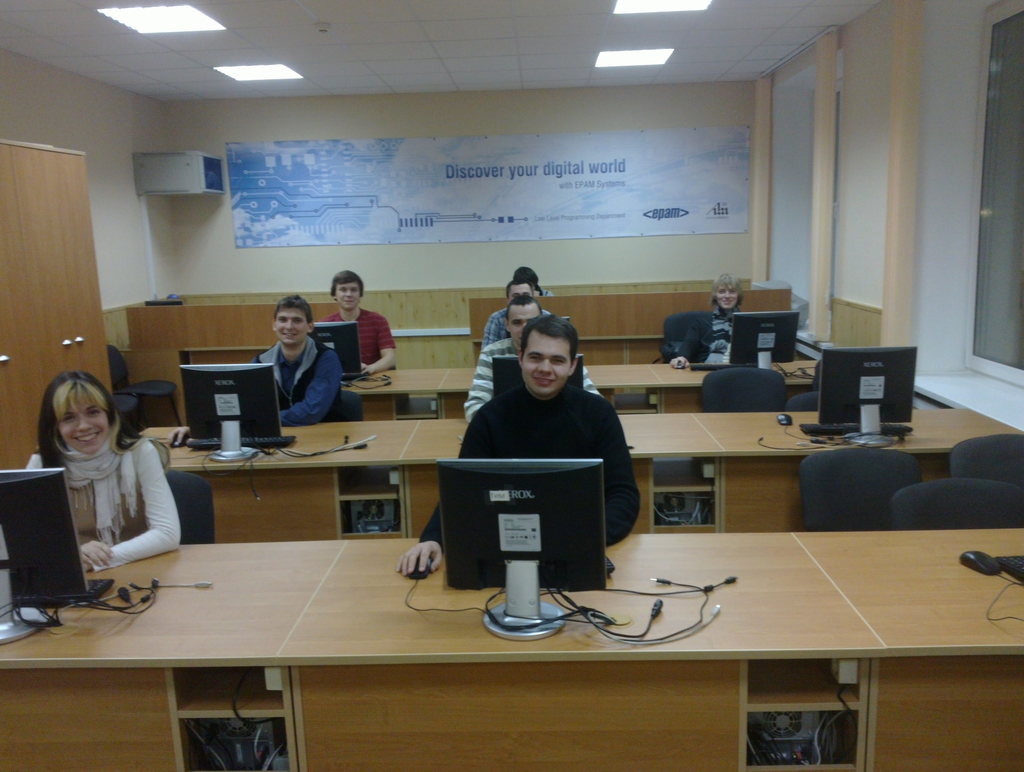
\includegraphics[height=0.5\textheight]{epam-evm_lab512}

	\begin{block}{Немного статистики}
		\begin{itemize}
			\item Подано заявок: {\bf 39} человек
			\item После первоначального отбора: {\bf 16} человек
				\begin{itemize}
					\item из них {\bf 4} -- сотрудники Epam
				\end{itemize}
		\end{itemize}
	\end{block}
\end{frame}

\begin{frame}
	\frametitle{Формат проведения занятий}

	\begin{block}{Принципы}
		\begin{itemize}
			\item Лекторы? Учителя? {\bf NO WAY!!!} 
				Разработчики для разработчиков! 
			\item Небольшая группа изучающих
			\item Балланс между теорией и практикой
		\end{itemize}
	\end{block}

	\pause

	\begin{block}{ $\beta$ -- версия: текущий статус}

		Все еще в \sout{разработке} процессе.

		\begin{itemize}
			\item Все планы нарушены ;-)
			\item 2 увлеченных человека
			\item Практически закончены 2 первых модуля
			\item Материалы выкладываются в общий доступ ``по-готовности''
				\begin{itemize}
					\item Патчи от студентов уже есть
				\end{itemize}
		\end{itemize}
	\end{block}

\end{frame}



